\begin{surferPage}[Chmutov]{Het achtstegraadsoppervlak van Chmutov}
    Een opvallend kenmerk van Chmutov's oppervlak van de graad 8 $\text{Chm}_{d}, \ d=8,$ is de symmetrie.
    We kunnen dit ook inzien door de vergelijking te onderzoeken:
    \[\text{Chm}_{d}\colon T_d(x) + T_d(y) + T_d(z) + 1 = 0,\]
     waar $T_d$ de zogenaamde Chebychev-veelterm voorstelt (afbeelding links).
    De kromme $T_8(x)+T_8(y)=0$ wordt rechts afgebeeld:
    
     \begin{center}
      \begin{tabular}{c@{\quad}c}
        \begin{tabular}{c}
          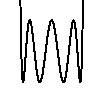
\includegraphics[height=1.75cm]{Tcheb_008.pdf}
        \end{tabular}    
        &
        \begin{tabular}{c}
          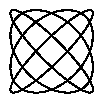
\includegraphics[height=1.75cm]{Tcheb_2d_008.pdf}
        \end{tabular}    
      \end{tabular}
    \end{center}
    \vspace{-0.3cm}
    Het is niet veel werk om van deze prentjes naar het interactieve oppervlak rechts over te gaan.


 S.V.\ Chmutov publiceerde deze vergelijkingen in de vroege jaren '80.
    Op dat moment hielden ze de wereldrecords voor $\mu(d)$ voor de meeste waarden van $d$.
    In de jaren '90 verbeterde Chmutov zijn eigen record, en in 2005 gebruikten S.~Breske,
    O.~Labs en D.~van~Straten zijn constructie ook voor re\"ele singulariteiten.
\end{surferPage}